\documentclass[12pt, letterpaper]{article}
\usepackage[margin=0.8in]{geometry}
\usepackage[utf8]{inputenc}
\usepackage[super,comma]{natbib}
\usepackage{graphicx}
\usepackage{xcolor}

\title{CMSC499A: Mutation Visualization}
\author{Mark Keller \thanks{mentored by Professor Max Leiserson}}
\date{Spring 2018}

\begin{document}
\maketitle

\begin{abstract}
Identification and analysis of patterns in data can be difficult without visualization tools. 
Datasets of somatic mutations in cancer are no exception.
Recent whole-genome sequencing projects such as PanCancer Analysis of Whole Genomes (PCAWG) have produced large amounts of data to be explored.
Of great importance is the classification of different mutational processes and the mutational signatures\cite{alexandrov2013signatures} they leave behind.
As new mutational signatures continue to be discovered, observation of the levels of signature activity, called signature exposure, helps show how the underlying mutational processes differ across cancer types, time, and environmental variables.
\end{abstract}

\section{Introduction}
Slight modifications to data sources used in past studies of mutations and mutation signatures have the potential to solidify or weaken conclusions made based on limited data.
For example, one might be interested in reproducing a past study across additional cancer types or in the context of additional variables, such as smoking status or age.
Web-based interactive visualizations allow for this type of comparison to be done across data sets and features in a way that is accessible and fast.
This semester, I have focused on building a visualization tool to do just this, using whole-genome somatic mutation datasets and mutation signature definitions from various sources.

The resulting tool, X (http://link.to/it), is a web-based mutation data browser that enables exploration of mutation signatures, cancer types, mutation types, and kataegis events.
X allows users to choose sequencing project data sets by cancer type, as well as mutation signature combinations (of which can be selected based on cancer-type-specific presets) before plotting this data. 
The following are types of plots that can be generated:
\begin{enumerate}
\item To illustrate estimated contributions of a selected combination of mutational signatures, a stacked bar plot can be generated, showing signature exposures for a sample, along with tobacco and alcohol usage indicators.
    Exposure values can be normalized to sum to one for each sample, or kept relative to the total number of mutations in each sample.
    This plot type was inspired by Figure 4 in Kim \textit{et al.} 2016 that displays estimated contributions of 4 different signatures and tobacco usage over cohorts of urothelial cancer tumor samples \cite{kim2016somatic}.
    \begin{figure}
        \caption{Signature Exposures with Clinical Variables}
        \centering
        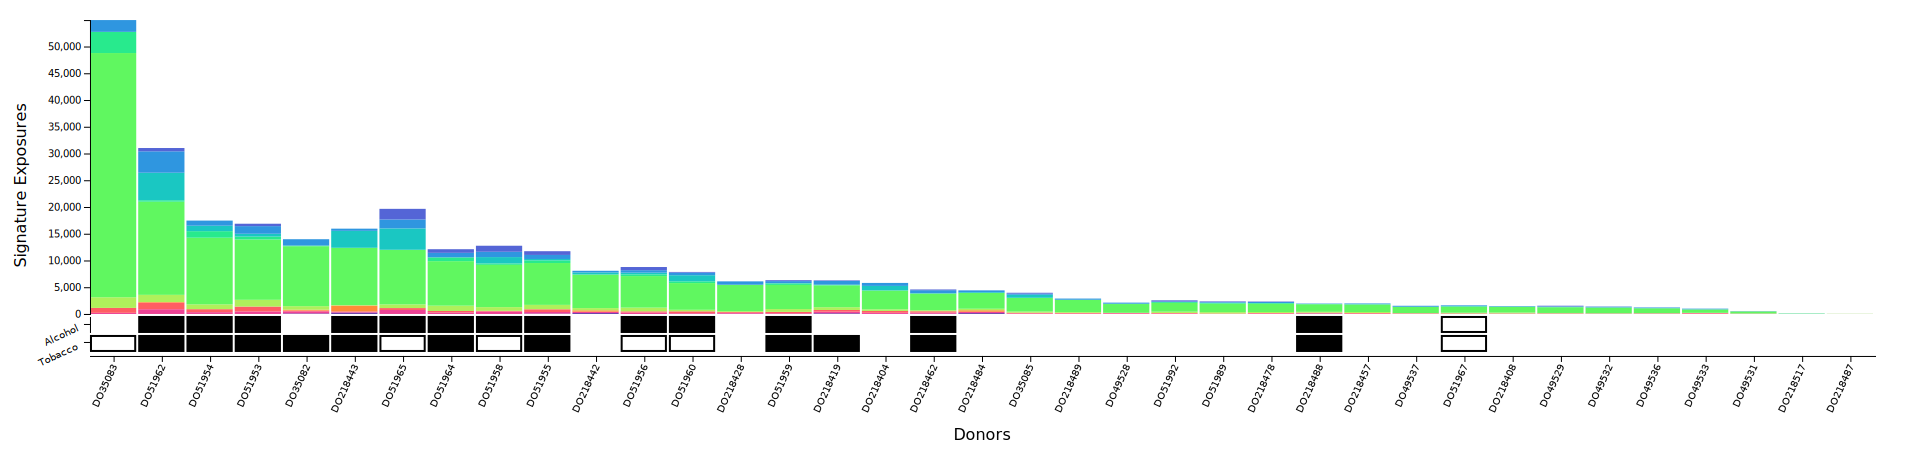
\includegraphics[width=\columnwidth]{figures/exposures.pdf}
    \end{figure}
\item To identify samples containing instances of localized hypermutation, called kataegis events, this second type of plot highlights kataegis events along the genome.
    Along the vertical axis are samples, and along the horizontal axis is the genome.
    Users can zoom and pan along each chromosome, and easily pinpoint kataegis events by the dark bars located on mutations in kataegis regions.
    Samples are grouped by sequencing project and cancer type.
    This plot doubles as a rainfall plot selector, as each sample bar can be clicked to generate a corresponding rainfall plot.
    To our knowledge, this style of plot has not been used before to visualize kataegis events.
    \begin{figure}
        \caption{Kataegis Plot}
        \centering
        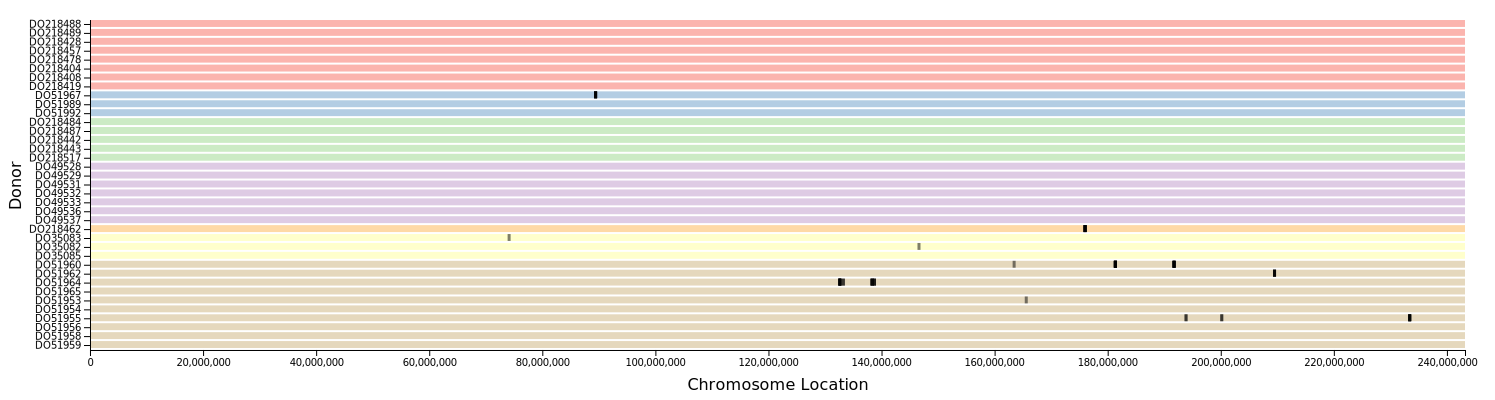
\includegraphics[width=\columnwidth]{figures/kataegis_chr2.pdf}
    \end{figure}
\item To examine mutation clusters, specifically those occurring in kataegis regions, a rainfall plot can be generated for each sample.
    Mutations are plotted horizontally based on their genome location, and vertically by the distance (in bp) to the previous mutation.
    Rainfall plots are commonly used to examine regions of hypermutation, as they allow these regions to be easily identified by vertical ``thunderbolts" of mutations. 
    This terminology is related to the name ``kataegis", which is derived from the Greek word for "thunder".
    Similar rainfall plots can be seen in Figure 4 of Nik-Zainal \textit{et al.} 2012\cite{nik2012mutational}.

    \begin{figure}
        \caption{Rainfall Plot}
        \centering
        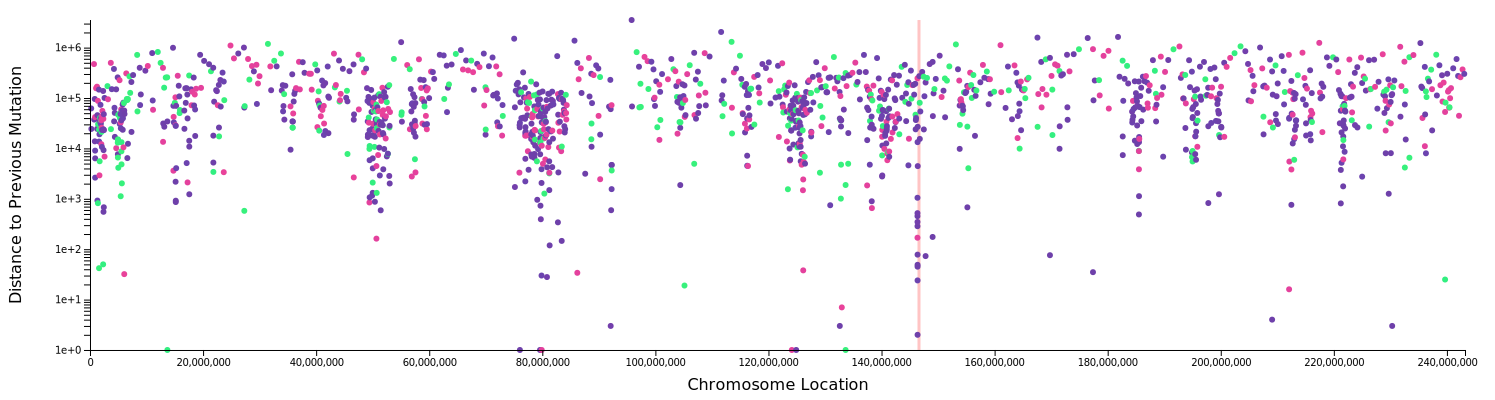
\includegraphics[width=\columnwidth]{figures/rainfall_DO35082_chr2.pdf}
    \end{figure}
\end{enumerate}







\section{Case Study}
This tool brings the power to visually analyze relationships between signature exposures and clinical variables.
Interactive sorting and dynamic calculations of signature exposures allow trends to be observed quickly.
Connections generally assumed to exist can be verified and examined, such as specific signatures being associated with tobacco usage.
Local datasets can be visualized, allowing functionality to extend beyond the public datasets we have processed.

\section{Methods}
Using the data-driven documents JavaScript library (D3.js)\cite{bostock2011d3}, each type of plot is tailored to suit the data types and data sets presented.
Showing donor clinical variables, such as smoking and alcohol usage, and their relationship to mutation signatures, requires this fine control that D3 provides.
In addition, D3 contains APIs for easy implementation of custom interactive features, such as highlighting, panning, and zooming.
Interactivity extends beyond single plots, linking plots together based on variables such as chromosome region and donor ID.   

This tool has been developed with maintainability and modularity in mind.
Using the Vue JavaScript framework, the application is made up of reusable components that encapsulate templates, functions, and variables.
Component state can be linked to events or ``watchers'' that observe and process data automatically upon change.
This functionality complements D3's ``dispatching''

\section{Future Directions}


\bibliography{main}{}
\bibliographystyle{plain}

\end{document}
